Was haben wir diese Woche gelernt? Um Aussagen über die Gitterstruktur eines Materials zu treffen, wird das Material in Frage mit monochromatischer
Röntgenstrahlung beleuchtet. Ein Anteil der eingebrachjten Röntgenstrahlung wird an Atomen innerhalb des Gitters gebeugt und kann mit passenden
Mitteln aufgefangen werden. Die so sichtbar gewordenen Muster sind charakteristisch für das jeweilige Kristallgitter, entsprechen ihm aber nicht
direkt. Was mir an dieser Stelle noch nicht ganz klar ist: sind das nun die reziproken Gitter? Oder sind sie nur ein mathematisches Hilfsmittel
zur Bestimmung der realen Gitter? Wie dem auch sei, die auf Folie 28 der VL präsentierte Formel stellt einen Zusammenhang zwischen Gangunterschied
der einstrahlenden Röntgenstrahlung und dem Abstand der Netzebenen her.
\begin{equation}
    n\lambda_{Röntgen} = 2\sin(\theta d_{hkl}) \vert n \in \mathbb{N}
    \label{eq:eq1}
\end{equation}

Hierbei sind \(n\) Vielfache der Wellenlänge und \(d_{hkl}\) der Abstand der Netzebenen definiert durch die miller'schen Indizes \(h\), \(k\) und \(l\).
Ich bin mir an dieser Stelle nicht ganz sicher, ob ich mich nicht ein wenig zu weit aus dem Fenster lehne. Ich glaube aber, dass Dr. Geberth hier einen
Bug eingebaut hat. Bei genauerer Betrachtung fällt auf, dass das Argument des Sinus die Einheit Meter besitzt. Der direkte Vergleich mit der Gleichung für
die Beugung am Gitter

\be
    n \lambda = d\sin(\alpha)
    \label{eq:eq2}
\ee

stützt diese These.\\

\textbf{Millersche Indizes}\\
Millersche Indizes - wie funktionieren sie? Wenn ich das korrekt verstanden habe und mich die Küchendiskusion darüber nicht im Stich lässt wird eine Ebene
definiert durch ihre Schnittpunkte mit den drei Raumachsen. Angegeben werden die Ortsvektoren der Schnittpunkte in Einheiten der Gitterkonstanten multipliziert
mit einem passenden Faktor. Nun wird der Kehrwert dieses Faktors gebildet und der kleinste gemeinsame Nenner aller drei Faktoren Gesucht. Voilá - die sich so
ergebenden Zähler sind die Miller-Indizes. Aus diesen Gedanken lässt sich auch direkt deduzieren wie ein Miller-Index aussieht, wenn die gesuchte Ebene keine
der Koordinatenachsen schneidet. In diesem Fall wird der entsprechende Koeffizient und damit auch sein Miller-Index null.\\

\textbf{Packungsdichte}\\
Die Packungsdichte ist für den Raum innerhalb einer Elementarzelle definiert. Sie ist das Verhältnis aus dem Volumen aller Atom-Teilvolumina innerhalb einer Zelle und dem
der Zelle selbst.

\begin{equation}
    PD = \frac{V_{Atom}}{V_{EZ}} \quad \vert \quad PD \in [0;1]
    \label{eq:eq3}
\end{equation}
    
Für den Fall kubisch-raumzentrierten Zelle (krz) wurde auf Folie 34 unter der Annahme, dass sich die Atomradien entlang der Würfeldiagonale berühren ein Wert
von 0,68 angegeben. Das sieht erstmal nach einer Behauptung aus und bedarf Investigation:\\

Mit
\begin{align*}
    4&r_{Atom} = \sqrt{3}a\\
    &r_{Atom} = \frac{\sqrt{3}}{4}a
\end{align*}
und der Tatsache, dass sich ein ganzes Atom in der Mitte befindet und jeweils ein achtel Atom von den Eckpunkten aus in den Raum ragt beträgt das Atomvolumen
\begin{align}
    V_{Atom} &= 8\frac{1}{8}+1(\frac{4}{3}\pi r_{Atom}^{3}) \nonumber\\
    &= \frac{8}{3}\pi (\frac{\sqrt{3}}{4}a)^{3} \nonumber\\
    &= \frac{\sqrt{3}}{8}\pi a^3
\end{align}
und eingesetzt in Gl. \ref{eq:eq3} die Packungsdichte für den Fall einer krz-Zelle (gerundet)
\be
    PD_{krz} = \frac{ \frac{ \sqrt{3} }{ 4 } \pi a^{3}}{ a^{3} } = 0,68
\ee
:)\\

Als weiteres Maß wird die Belegungsdichte \(BD\) genannt. Sie ist definiert als das Verhältnis der Schnittflächen der Atome zu der Schnittfläche der Elementarzelle.
Bildlich ist sich das vorzustellen wie ein m\&m-Kuchen unter einer Guillotine. Schaue ich mir die Schnittfläche an kann ich ein Verhältnis von erwischten m\&m zum umgebenden Kuchenteig bilden.
Es wurde behauptet, dass entlang der Ebene {110} die höchste Belegungsdichte sei.\\
\begin{wrapfigure}{r}{5cm}
    \centering
    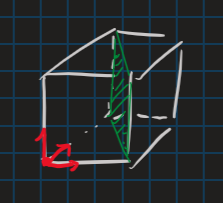
\includegraphics[scale=0.7]{entries/\eintrag/110.png}
    \caption{Rot: Koordinatenursprung, Grün: Schnittebene}
    \label{fig:110}
\end{wrapfigure}
Es ist recht eingängig, dass hier aus den anliegenden Eckpunkten jeweils ein Viertel einer Kreisfläche in die Schnittebene ragt und zusätzlich noch eine ganze Kreisfläche in der Mitte liegt.
Ähnlich dem Vorgehen für das Volumen lassen sich hier Gleichungen herleiten und

\begin{align*}
    r_{Atom} = \frac{\sqrt{3}}{4}a && BD_{kfz}&=\frac{2\pi r_{Atom}^2}{\sqrt{2}a^2}\\
    && &=\frac{6\pi}{16\sqrt{2}}\\
    && &=0,833
\end{align*}

die Behauptung muss keine bleiben.\\

Für die kfz-Zelle (kubisch flächenzentriert) funktioniert das ganz analog. Hier befindet sich in der Mitte jeder Würfelfläche und an jedem Eckpunkt ein Atom, keines aber in der Mitte.
In den Raum ragen nun wieder die gleichen acht Achtel Atome und zusätzlich noch sechs Atomhälften. Die Atomradien berühren sich hier entlang der Flächendiagonalen.\\

\textbf{Reale Strukturen}\\
Bisher wurden ideale Strukturen i.e. homogene Kristalle betrachtet. In der echten Welt sind aber viele Arten von Defekten zu finden. Die gesamte Halbleiterindustrie basiert auf gezielt
eingebrachten Defekten in Kristallstrukturen. In Metallen und ihren Legierungen befinden sich zwar nicht derart hochtechnologisch eingebrachte Defekte aber auch hier können und werden sie
gezielt ausgenutzt um bestimmte Materialeigenschaften ein zu stellen.

Grundsätzlich werden hier Defekte geometrischen unterschieden.
\begin{itemize}
    \item Nulldimensional - Defekte, die sich auf einzelne Stellen im Kristall beschränken. Etwa eine falsch oder unbesetzte Stelle.
    \item Eindimensional - verstanden habe ich das, als würde eine steife Perlenkette in eine periodisch aufgebaute Masse aus anderen Perlen getrieben werden. Unmittelbar um die Perlenkette
    ist die Masse verdichtet/verformt was zu graduellen unregelmäßigkeiten des Gitters führt.
    \item Zweidimensional - Deplatzierungen einer oder mehrerer Gitterebenen.
    \item Dreidimensional - Häufung Nulldimensionaler Bugs
    \item Korn/Phasengrenzen
\end{itemize}

Letztere sind so etwas wie Bezirke nahezu homogener Struktur innerhalb eines Kristalls.

Memo an mich selbst: übe TikZ!